% Options for packages loaded elsewhere
\PassOptionsToPackage{unicode}{hyperref}
\PassOptionsToPackage{hyphens}{url}
%
\documentclass[
]{book}
\usepackage{amsmath,amssymb}
\usepackage{iftex}
\ifPDFTeX
  \usepackage[T1]{fontenc}
  \usepackage[utf8]{inputenc}
  \usepackage{textcomp} % provide euro and other symbols
\else % if luatex or xetex
  \usepackage{unicode-math} % this also loads fontspec
  \defaultfontfeatures{Scale=MatchLowercase}
  \defaultfontfeatures[\rmfamily]{Ligatures=TeX,Scale=1}
\fi
\usepackage{lmodern}
\ifPDFTeX\else
  % xetex/luatex font selection
\fi
% Use upquote if available, for straight quotes in verbatim environments
\IfFileExists{upquote.sty}{\usepackage{upquote}}{}
\IfFileExists{microtype.sty}{% use microtype if available
  \usepackage[]{microtype}
  \UseMicrotypeSet[protrusion]{basicmath} % disable protrusion for tt fonts
}{}
\makeatletter
\@ifundefined{KOMAClassName}{% if non-KOMA class
  \IfFileExists{parskip.sty}{%
    \usepackage{parskip}
  }{% else
    \setlength{\parindent}{0pt}
    \setlength{\parskip}{6pt plus 2pt minus 1pt}}
}{% if KOMA class
  \KOMAoptions{parskip=half}}
\makeatother
\usepackage{xcolor}
\usepackage{color}
\usepackage{fancyvrb}
\newcommand{\VerbBar}{|}
\newcommand{\VERB}{\Verb[commandchars=\\\{\}]}
\DefineVerbatimEnvironment{Highlighting}{Verbatim}{commandchars=\\\{\}}
% Add ',fontsize=\small' for more characters per line
\usepackage{framed}
\definecolor{shadecolor}{RGB}{248,248,248}
\newenvironment{Shaded}{\begin{snugshade}}{\end{snugshade}}
\newcommand{\AlertTok}[1]{\textcolor[rgb]{0.94,0.16,0.16}{#1}}
\newcommand{\AnnotationTok}[1]{\textcolor[rgb]{0.56,0.35,0.01}{\textbf{\textit{#1}}}}
\newcommand{\AttributeTok}[1]{\textcolor[rgb]{0.13,0.29,0.53}{#1}}
\newcommand{\BaseNTok}[1]{\textcolor[rgb]{0.00,0.00,0.81}{#1}}
\newcommand{\BuiltInTok}[1]{#1}
\newcommand{\CharTok}[1]{\textcolor[rgb]{0.31,0.60,0.02}{#1}}
\newcommand{\CommentTok}[1]{\textcolor[rgb]{0.56,0.35,0.01}{\textit{#1}}}
\newcommand{\CommentVarTok}[1]{\textcolor[rgb]{0.56,0.35,0.01}{\textbf{\textit{#1}}}}
\newcommand{\ConstantTok}[1]{\textcolor[rgb]{0.56,0.35,0.01}{#1}}
\newcommand{\ControlFlowTok}[1]{\textcolor[rgb]{0.13,0.29,0.53}{\textbf{#1}}}
\newcommand{\DataTypeTok}[1]{\textcolor[rgb]{0.13,0.29,0.53}{#1}}
\newcommand{\DecValTok}[1]{\textcolor[rgb]{0.00,0.00,0.81}{#1}}
\newcommand{\DocumentationTok}[1]{\textcolor[rgb]{0.56,0.35,0.01}{\textbf{\textit{#1}}}}
\newcommand{\ErrorTok}[1]{\textcolor[rgb]{0.64,0.00,0.00}{\textbf{#1}}}
\newcommand{\ExtensionTok}[1]{#1}
\newcommand{\FloatTok}[1]{\textcolor[rgb]{0.00,0.00,0.81}{#1}}
\newcommand{\FunctionTok}[1]{\textcolor[rgb]{0.13,0.29,0.53}{\textbf{#1}}}
\newcommand{\ImportTok}[1]{#1}
\newcommand{\InformationTok}[1]{\textcolor[rgb]{0.56,0.35,0.01}{\textbf{\textit{#1}}}}
\newcommand{\KeywordTok}[1]{\textcolor[rgb]{0.13,0.29,0.53}{\textbf{#1}}}
\newcommand{\NormalTok}[1]{#1}
\newcommand{\OperatorTok}[1]{\textcolor[rgb]{0.81,0.36,0.00}{\textbf{#1}}}
\newcommand{\OtherTok}[1]{\textcolor[rgb]{0.56,0.35,0.01}{#1}}
\newcommand{\PreprocessorTok}[1]{\textcolor[rgb]{0.56,0.35,0.01}{\textit{#1}}}
\newcommand{\RegionMarkerTok}[1]{#1}
\newcommand{\SpecialCharTok}[1]{\textcolor[rgb]{0.81,0.36,0.00}{\textbf{#1}}}
\newcommand{\SpecialStringTok}[1]{\textcolor[rgb]{0.31,0.60,0.02}{#1}}
\newcommand{\StringTok}[1]{\textcolor[rgb]{0.31,0.60,0.02}{#1}}
\newcommand{\VariableTok}[1]{\textcolor[rgb]{0.00,0.00,0.00}{#1}}
\newcommand{\VerbatimStringTok}[1]{\textcolor[rgb]{0.31,0.60,0.02}{#1}}
\newcommand{\WarningTok}[1]{\textcolor[rgb]{0.56,0.35,0.01}{\textbf{\textit{#1}}}}
\usepackage{longtable,booktabs,array}
\usepackage{calc} % for calculating minipage widths
% Correct order of tables after \paragraph or \subparagraph
\usepackage{etoolbox}
\makeatletter
\patchcmd\longtable{\par}{\if@noskipsec\mbox{}\fi\par}{}{}
\makeatother
% Allow footnotes in longtable head/foot
\IfFileExists{footnotehyper.sty}{\usepackage{footnotehyper}}{\usepackage{footnote}}
\makesavenoteenv{longtable}
\usepackage{graphicx}
\makeatletter
\def\maxwidth{\ifdim\Gin@nat@width>\linewidth\linewidth\else\Gin@nat@width\fi}
\def\maxheight{\ifdim\Gin@nat@height>\textheight\textheight\else\Gin@nat@height\fi}
\makeatother
% Scale images if necessary, so that they will not overflow the page
% margins by default, and it is still possible to overwrite the defaults
% using explicit options in \includegraphics[width, height, ...]{}
\setkeys{Gin}{width=\maxwidth,height=\maxheight,keepaspectratio}
% Set default figure placement to htbp
\makeatletter
\def\fps@figure{htbp}
\makeatother
\setlength{\emergencystretch}{3em} % prevent overfull lines
\providecommand{\tightlist}{%
  \setlength{\itemsep}{0pt}\setlength{\parskip}{0pt}}
\setcounter{secnumdepth}{5}
\usepackage{booktabs}
\ifLuaTeX
  \usepackage{selnolig}  % disable illegal ligatures
\fi
\usepackage[]{natbib}
\bibliographystyle{apalike}
\IfFileExists{bookmark.sty}{\usepackage{bookmark}}{\usepackage{hyperref}}
\IfFileExists{xurl.sty}{\usepackage{xurl}}{} % add URL line breaks if available
\urlstyle{same}
\hypersetup{
  pdftitle={GitHub for Public Health},
  pdfauthor={Corinne Riddell and Lauren Wilner},
  hidelinks,
  pdfcreator={LaTeX via pandoc}}

\title{GitHub for Public Health}
\author{Corinne Riddell and Lauren Wilner}
\date{2024-04-19}

\begin{document}
\maketitle

{
\setcounter{tocdepth}{1}
\tableofcontents
}
\hypertarget{about-this-training}{%
\chapter{About this training}\label{about-this-training}}

Keeping track of changes to your statistical code can really help cut down on mistakes in your analysis. But, a lot of epidemiologists haven't been trained on how to do this, and might wonder how it all fits with IRB protocols and privacy rules. In these materials, we get into the basics of git and GitHub. We'll show you how these tools can help you manage your code changes safely and ethically.
LBW Note: is this the right tone?

\textbf{Questions? Comments?}

Contact us at \href{mailto:datasci.ph@gmail.com}{\nolinkurl{datasci.ph@gmail.com}} if you have questions, comments, or feedback!

\hypertarget{workshop-setup}{%
\chapter{Workshop Setup}\label{workshop-setup}}

This pre-workshop guide is designed to walk you through the initial setup of git on your computer.

If you have any issues, please reach out to us at \href{mailto:datasci.ph@gmail.com}{\nolinkurl{datasci.ph@gmail.com}}.

\textbf{Introduction}

Git is a version control system that allows you to track changes in your code.

In order to get setup, we need to install git on your computer, make a GitHub account, and configure git on your computer.

We will get into the details of how to use git in the workshop, but are requesting that you complete the following steps before the workshop so that we can spend all of the workshop time on using Git rather than on setup!

\hypertarget{install-r-and-rstudio-if-you-have-not-already}{%
\section{Install R and RStudio if you have not already:}\label{install-r-and-rstudio-if-you-have-not-already}}

\begin{itemize}
\tightlist
\item
  \url{https://posit.co/download/rstudio-desktop/}
\end{itemize}

\hypertarget{open-rstudio-and-install-the-following-packages}{%
\section{Open RStudio and install the following packages:}\label{open-rstudio-and-install-the-following-packages}}

\begin{itemize}
\tightlist
\item
  \textbf{tidyverse}
\item
  \textbf{usethis}
\item
  \textbf{gitcreds}
\item
  \textbf{broom}
\end{itemize}

To do this, run the following code in the RStudio console:
\texttt{install.packages(\textquotesingle{}tidyverse\textquotesingle{})}
Do this for each of the packages.

\emph{If any of these packages fail to install, please let us know. You may need to update your RStudio but we will try to help you get everything set up with minimal interruption to your other work.}

\hypertarget{create-a-github-account}{%
\section{Create a github account}\label{create-a-github-account}}

\begin{itemize}
\tightlist
\item
  \url{https://github.com/}
\end{itemize}

\hypertarget{install-git}{%
\section{Install Git}\label{install-git}}

Follow the instructions on the following slides to install git on your computer. Select the slides that correspond to Windows or Mac depending on what machine you are using.

\hypertarget{windows-instructions}{%
\subsection{Windows Instructions}\label{windows-instructions}}

\begin{enumerate}
\def\labelenumi{\arabic{enumi})}
\tightlist
\item
  Download Git for Windows from here: \url{https://gitforwindows.org/}. There are lots of things to click through.
\end{enumerate}

Notes from HappyGitWithR:
NOTE: When asked about ``Adjusting your PATH environment'', make sure to select ``Git from the command line and also from 3rd-party software''. Otherwise, we believe it is good to accept the defaults.
Note that RStudio for Windows prefers for Git to be installed below C:/Program Files and this appears to be the default. This implies, for example, that the Git executable on my Windows system is found at C:/Program Files/Git/bin/git.exe. Unless you have specific reasons to otherwise, follow this convention.

\begin{enumerate}
\def\labelenumi{\arabic{enumi})}
\setcounter{enumi}{1}
\item
  Start menu \textgreater{} Git \textgreater{} Git Bash. Confirm that you have access to Git Bash.
\item
  RStudio next
  RStudio should automatically detect the presence of Git Bash. You can inspect and influence this directly via Tools \textgreater{} Global Options \textgreater{} Terminal. Unless you have good reason to do otherwise, you want to see ``Git Bash'' in the ``New terminals open with \ldots{}'' dropdown menu.
\item
  The next set of tasks are done in RStudio. The code to run these commands are found in the file \texttt{code/00\_Setup-instructions-for-Windows.R}. After running all those commands you are ready to use GitHub from the Shell. (Currently, these instructions do not include setting up a Git client.)
\end{enumerate}

(\url{https://youtu.be/0blgUPi5j4U})

\hypertarget{mac-instructions}{%
\subsection{Mac Instructions}\label{mac-instructions}}

\begin{enumerate}
\def\labelenumi{\arabic{enumi})}
\tightlist
\item
  Type git --version in your terminal to check if git is installed. If it is, you will see a version number. If not, type:
  \texttt{git\ config} and then \texttt{enter}. You will be prompted to install Git and follow the prompts!
\end{enumerate}

\hypertarget{configure-git-using-an-https-token}{%
\section{Configure Git using an HTTPS token}\label{configure-git-using-an-https-token}}

Load \texttt{usethis} \& \texttt{gitcreds}:

\begin{itemize}
\tightlist
\item
  \texttt{library(usethis)}
\item
  \texttt{library(gitcreds)}
\end{itemize}

Pick a user name - it does not need to be your GitHub user name. This is the email address linked to your GitHub account:\\
\texttt{use\_git\_config(user.name\ =\ "Corinne\ Riddell\ on\ Dell",}
\texttt{user.email\ =\ "corinne.riddell@gmail.com")}

After you have installed the packages, you will need to create a personal access token. This is a way to authenticate yourself with GitHub. You will need to do this in order to push and pull from your repository. Run the following:

\texttt{usethis::create\_github\_token()}

This will bring you to a browser page. Put in a description for your token and then select an expiration date from the drop down - please select \texttt{No\ expiration}. Scroll down and click the \texttt{Generate\ token} button. Copy the token that is generated and paste it somewhere where you will be able to access it.

Go back to R and run the following:

\texttt{gitcreds::gitcreds\_set()}

When prompted, paste in the token you copied. This will add your credentials to your cache. The following will print out to the RStudio console:

\texttt{?\ Enter\ password\ or\ token:\ ghp\_xxxxxxxxxxxxxxxxxxxxxxxxxxxxxxxxxxxx}\strut \\
\texttt{-\textgreater{}\ Adding\ new\ credentials...}\strut \\
\texttt{-\textgreater{}\ Removing\ credentials\ from\ cache...}\strut \\
\texttt{-\textgreater{}\ Done.}

(\url{https://youtu.be/yedGFJifmdI})

\hypertarget{resources}{%
\section{Resources}\label{resources}}

You should now be set up to use Git and Github! If you had any issues, here are a few links you can look at for help. If you are still having trouble, please reach out to us before the workshop!

\begin{itemize}
\item
  \href{https://happygitwithr.com/}{Happy Git with R}
\item
  \href{https://git-scm.com/book/en/v2/Getting-Started-About-Version-ControlLinks}{Git Setup Book}
\end{itemize}

\hypertarget{why-git-and-github}{%
\chapter{Why Git and GitHub}\label{why-git-and-github}}

\hypertarget{what-is-version-control-git-and-github}{%
\section{What is version control, Git, and Github?}\label{what-is-version-control-git-and-github}}

\begin{itemize}
\tightlist
\item
  \textbf{Version control} is the practice of tracking and managing changes to
  (statistical) code and other files.
\item
  \textbf{Git} is a version control system. It tracks what is changed in a file,
  when and by whom and synchronizes the changes to a central server so that multiple
  contributors can manage changes to the same set of files (Wilson et al., 2017).
\item
  \textbf{GitHub} is a hosting service on the web for Git repositories.
  Reference: Wilson G, et al.~Good enough practices in scientific computing. PLoS Comp Bio. 2017.
\end{itemize}

\hypertarget{the-case-for-version-control}{%
\section{The case for version control}\label{the-case-for-version-control}}

\hypertarget{error-reducing}{%
\subsection{Error reducing}\label{error-reducing}}

\begin{itemize}
\tightlist
\item
  Version control \textbf{eliminates} the need to send code or outputs (graphics,
  reports) via email or share folders between collaborators. With a version
  control system, everyone has access to the most recent set of files.
\end{itemize}

\hypertarget{version-control-facilitates-reproducible-analyses}{%
\subsection{Version control facilitates reproducible analyses}\label{version-control-facilitates-reproducible-analyses}}

\begin{itemize}
\tightlist
\item
  Have you ever tried to reproduce an analysis you did 3 years ago?
\item
  Have you ever tried to reproduce someone else's analysis?

  \begin{itemize}
  \tightlist
  \item
    Their links don't work on your computer
  \item
    You may or may not have access to the data
  \end{itemize}
\end{itemize}

\hypertarget{version-control-facilitates-reproducible-analyses-1}{%
\subsection{Version control facilitates reproducible analyses}\label{version-control-facilitates-reproducible-analyses-1}}

\begin{itemize}
\tightlist
\item
  Because everyone has access to the same files, a project's workflow can be set up
  to ensures that the analyses are reproducible for everyone.
\item
  In R, this can be as simple as hitting the ``knit'' button to run the analyses
  on anyone's computer -- no need to update the file pathways, no need to download
  new versions of the code or data.
\end{itemize}

\hypertarget{makes-supervision-and-collaboration-easier}{%
\subsection{Makes supervision and collaboration easier}\label{makes-supervision-and-collaboration-easier}}

\begin{itemize}
\tightlist
\item
  With Github, you can easily view changes made to statistical code. So if
  you are working together, it is easy to tell what lines of code were changed,
  alongside downstream changes to reports or data visualizations as a result of the
  change to the analysis.
\end{itemize}

\hypertarget{rollback-capabilities}{%
\subsection{Rollback capabilities}\label{rollback-capabilities}}

\begin{itemize}
\tightlist
\item
  You can use Git to roll back to a previous version of a file at any point. To do this, you would search for the \texttt{commit\ ID} of the version you want to revert to and then use the \texttt{git\ checkout\ \{commit\ ID\}} command to revert to that version. This is useful if your team decides that a change made to the code was not beneficial or wants to revert back to a different strategy that was used previously.
\end{itemize}

\hypertarget{github-supports-expeditious-sharing-of-scientific-approaches-and-findings}{%
\subsection{Github supports expeditious sharing of scientific approaches and findings}\label{github-supports-expeditious-sharing-of-scientific-approaches-and-findings}}

\begin{itemize}
\tightlist
\item
  Anything posted on GitHub can be shared widely to your organization or with
  the public.
\end{itemize}

\hypertarget{git-jargon-alice-bartlett}{%
\chapter{Git Jargon (Alice Bartlett)}\label{git-jargon-alice-bartlett}}

Write a blurb about Alice's slides, link her slides, show screenshot of first slide.

\hypertarget{setup-of-solo-workflow}{%
\chapter{Setup of Solo Workflow}\label{setup-of-solo-workflow}}

\hypertarget{outline-for-this-section}{%
\section{Outline for this section}\label{outline-for-this-section}}

We have discussed why Git and GitHub are important, now we will set up a repository and work through an example. During this first section, you will be working in a repository alone. We will:

\begin{itemize}
\tightlist
\item
  Make a new repository on GitHub\\
\item
  Clone the repository to your local machine\\
\item
  Write code in your repository locally\\
\item
  Push the code to your repository\\
\item
  Merge your branch into main
\end{itemize}

\hypertarget{working-in-terminal-mac-and-bash-windows}{%
\section{Working in Terminal (Mac) and Bash (Windows)}\label{working-in-terminal-mac-and-bash-windows}}

\begin{itemize}
\tightlist
\item
  We will use Terminal and Bash applications to interact with Git on our laptops.
\item
  Below is a Mac Terminal window. It looks very similar to a Windows Bash window.
\end{itemize}

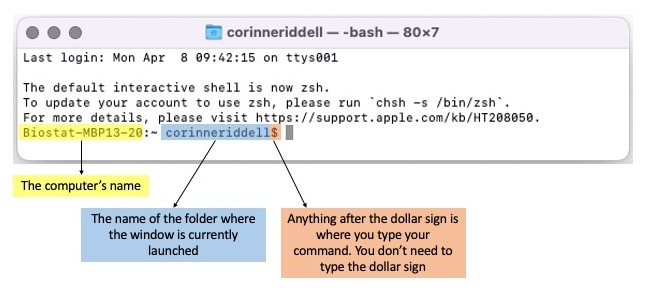
\includegraphics[width=1\linewidth]{./figures/Terminal-explainer-1}

\begin{itemize}
\tightlist
\item
  In this session, we will supply you with Git code for you to manually input
  into your Terminal/Bash windows. Note that all of this code will be written after
  the dollar sign in the figure above.
\end{itemize}

\hypertarget{working-in-terminal-mac-and-bash-windows-1}{%
\section{Working in Terminal (Mac) and Bash (Windows)}\label{working-in-terminal-mac-and-bash-windows-1}}

\begin{itemize}
\tightlist
\item
  Here is an example of the command \texttt{git\ branch}, followed by the output printed
  to screen:
\end{itemize}

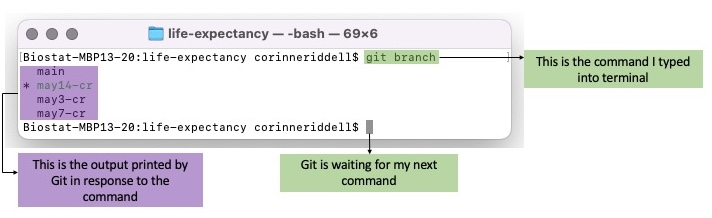
\includegraphics[width=1\linewidth]{./figures/Terminal-explainer-2}

\hypertarget{folder-names-and-file-names-tips}{%
\section{Folder names and file names tips}\label{folder-names-and-file-names-tips}}

\begin{itemize}
\tightlist
\item
  Recall when you name a variable in SAS or R, the variable name cannot
  contain spaces or unusual characters.
\item
  It is best practice to not use spaces or unusual characters in folder
  or file names, even though spaces are permissible and commonly used by Windows
  and Mac Users.
\end{itemize}

\hypertarget{good-folder-names}{%
\section{Good folder names\ldots{}}\label{good-folder-names}}

\begin{itemize}
\tightlist
\item
  Use dashes in place of spaces
\item
  Use capitalization instead of spaces
\end{itemize}

\hypertarget{good-folder-names-examples}{%
\subsection{Good folder names examples}\label{good-folder-names-examples}}

\begin{itemize}
\tightlist
\item
  life-expectancy
\item
  lifeExpectancy
\item
  LifeExpectancy
\end{itemize}

\hypertarget{what-is-the-problem-with-spaces-anyway}{%
\section{What is the problem with spaces, anyway?}\label{what-is-the-problem-with-spaces-anyway}}

\begin{itemize}
\tightlist
\item
  While spaces are human-readable they aren't machine-friendly.
\item
  When you refer to a folder or file using Git in Terminal or Bash, a name
  without spaces is much easier to type (otherwise you have to insert a
  backslash before the space)
\item
  Spaces also break the auto-complete function that Git users love. This is a
  very frustrating experience.
\end{itemize}

\hypertarget{good-file-names-are}{%
\section{Good file names are\ldots{}}\label{good-file-names-are}}

\begin{itemize}
\tightlist
\item
  machine readable
\item
  human readable
\item
  play well with default ordering
\end{itemize}

See the file ``how-to-name-files.pdf'' for a more deeper dive into file naming.

\hypertarget{good-file-names-examples}{%
\subsection{Good file names examples}\label{good-file-names-examples}}

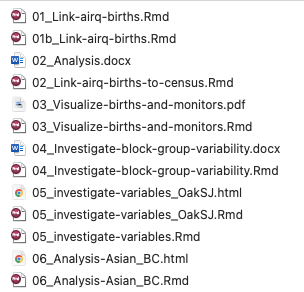
\includegraphics[width=0.75\linewidth]{./figures/Variable-names-example}

\begin{itemize}
\tightlist
\item
  Filenames start with a number (padded by 0) to order the files according to
  the order performed in the analysis
\item
  This is followed by a short (human and machine readable) descriptor of what
  the file does
\item
  Uses underscore ``\_'' to delimit field, and dashes ``-'' to separate words within field
\end{itemize}

\hypertarget{bad-file-name-example-and-associated-git-pain}{%
\subsection{Bad file name example (and associated Git pain)}\label{bad-file-name-example-and-associated-git-pain}}

\begin{itemize}
\tightlist
\item
  Can see that there is an R markdown (Rmd) file named ``Data Visualization Evaluation Report'' that has been modified.
\item
  The pain arises when I go to \texttt{git\ add} the file. Before each space, I need to
  include a backslash (which looks ugly). Even worse, the space breaks the auto-complete that happens when I press ``tab'' to auto-complete the file name.
  Auto-complete will become your friend when you use Git, and not being able to
  use it is very sad/infuriating when you have grown to love it.
\end{itemize}

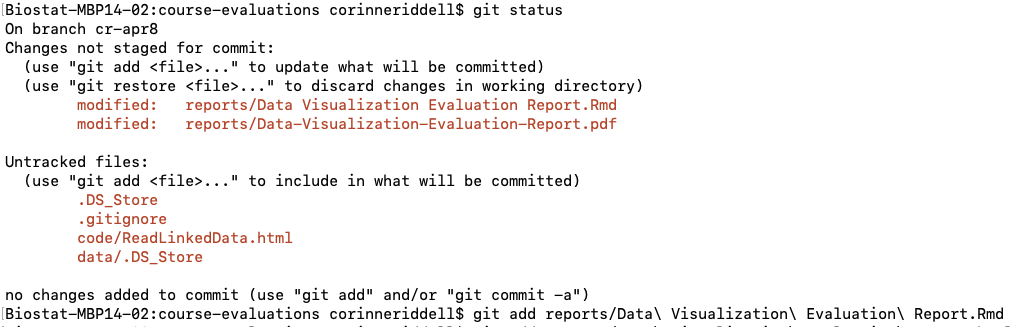
\includegraphics[width=1\linewidth]{./figures/Space-in-pathways-pain}

\hypertarget{set-up-a-project-that-you-want-to-track-with-git-and-github}{%
\section{Set up a project that you want to track with git and GitHub}\label{set-up-a-project-that-you-want-to-track-with-git-and-github}}

Let's suppose that you have a project that you want to start tracking using Git
and Github. For this project, you are already working on with some code, data,
and visualizations that have already been saved. We have made this project for
you. To download it, run the following two commands in the RStudio console:

\begin{Shaded}
\begin{Highlighting}[]
\FunctionTok{install.packages}\NormalTok{(}\StringTok{"usethis"}\NormalTok{)}
\NormalTok{usethis}\SpecialCharTok{::}\FunctionTok{use\_course}\NormalTok{(}\StringTok{"corinne{-}riddell/existing{-}project"}\NormalTok{)}
\end{Highlighting}
\end{Shaded}

\begin{itemize}
\tightlist
\item
  R will asked you if you want this folder copied onto the Desktop. Select Yes.
\item
  R will display messages showing you that the folder has been downloaded and unzipped.
  Tell R whether to delete the file.
\item
  RStudio will then open. Click the code folder in the file viewer. Then, click
  the filename ``01\_Analyze-life-expectancy.R'' to open this file in RStudio.
\item
  Run all the code in the .R file you just downloaded. Note that it created a figure and
  saved it into the images sub-folder.
\end{itemize}

Now you are set up with some existing code and things that you might want to start
tracking on GitHub. The next thing to do is make a folder on GitHub that will
store this project.

\hypertarget{make-a-new-repository-on-github}{%
\section{Make a new repository on GitHub}\label{make-a-new-repository-on-github}}

\begin{itemize}
\tightlist
\item
  Go to github.com and log in. Click the green ``New'' button to make a GitHub
  repository. Type ``life-expectancy'' in the repository name.
\item
  Write whatever you want in the description. For example, type ``An analysis of life expectancy in the US''
\item
  Select either to make this a public or private repository.
\item
  Check the box next to \texttt{Add\ a\ README\ file}. This tells Git to create a file that can describe your project. For now, you can write a sentence about this being a practice repository for this workshop.\\
\item
  Choose \texttt{.gitignore} template: \texttt{R}. This tells Git to use defaults that work well for R users.\\
\item
  Choose \texttt{MIT\ License}. This relates to the licensing for your code, which is not relevant for this workshop.\\
\item
  Click ``Create repository''. Github will then bring you to the repository's
  main page.
\end{itemize}

\hypertarget{clone-the-repository-to-your-local-machine}{%
\section{Clone the repository to your local machine}\label{clone-the-repository-to-your-local-machine}}

\begin{itemize}
\tightlist
\item
  From the main page of your repository and click on the green \texttt{Code} button.\\
\item
  You'll see a URL that starts with \url{https://}. Push the icon with two overlapping
  squares to copy the URL to your clipboard. {[}Lauren, you had written this differently and had them use the SSH one\ldots{} is there a reason to use one over the other?{]}
\item
  Open terminal (Mac) or bash (Windows) program. Navigate to where you want to place
  this repository using the \texttt{cd\ \{folder\_name\}} command. Then write
  \texttt{git\ clone\ \{paste\ the\ url\ you\ copied\ here\}} and
  then press the return/enter button. The following will display in Terminal/Bash
  if this was successful:
\end{itemize}

\begin{verbatim}
Biostat-MBP13-20:repos corinneriddell$ git clone https://github.com/corinne-riddell/life-expectancy.git

Cloning into 'life-expectancy'...
remote: Enumerating objects: 5, done.
remote: Counting objects: 100% (5/5), done.
remote: Compressing objects: 100% (5/5), done.
remote: Total 5 (delta 0), reused 0 (delta 0), pack-reused 0
Unpacking objects: 100% (5/5), done.
\end{verbatim}

You now are ready to begin tracking changes to this folder using Git and GitHub.

\hypertarget{get-oriented-to-the-new-directory}{%
\section{Get oriented to the new directory}\label{get-oriented-to-the-new-directory}}

To get yourself oriented, do the following in the Terminal/Bash window:

\begin{itemize}
\tightlist
\item
  Navigate into your repository by typing \texttt{cd\ life-expectancy/}.
\item
  Type \texttt{git\ status}. The results shows you that no changes have been made yet:
\end{itemize}

\begin{verbatim}
Biostat-MBP13-20:life-expectancy corinneriddell$git status
On branch main
Your branch is up to date with 'origin/main'.

nothing to commit, working tree clean
\end{verbatim}

\begin{itemize}
\tightlist
\item
  Type \texttt{git\ branch}. This shows you that you are currently on the main branch.
\end{itemize}

\begin{verbatim}
Biostat-MBP13-20:life-expectancy corinneriddell$git branch
* main
\end{verbatim}

\hypertarget{make-your-first-branch}{%
\section{Make your first branch}\label{make-your-first-branch}}

Set yourself up in a new branch off of main. In terminal/bash:

\begin{itemize}
\tightlist
\item
  Type \texttt{git\ checkout\ -b\ may3-XY}, replacing XY with your initials. (If today
  is not May 3, replace ``may3'' with today's date.)
\end{itemize}

\begin{verbatim}
Biostat-MBP13-20:life-expectancy corinneriddell$ git checkout -b may3-cr
Switched to a new branch 'may3-cr'
\end{verbatim}

\begin{itemize}
\tightlist
\item
  Type \texttt{git\ branch}, to confirm to yourself that you have indeed switched to
  the new branch.
\end{itemize}

\begin{verbatim}
Biostat-MBP13-20:life-expectancy corinneriddell$ git branch
  main
* may3-cr
\end{verbatim}

\hypertarget{make-some-changes-to-your-code}{%
\section{Make some changes to your code}\label{make-some-changes-to-your-code}}

Okay, you are now set up to track changes. Let's do the following:

\begin{itemize}
\tightlist
\item
  Copy the code/ data/ and images/ sub-folders from your ``existing-project'' folder into the
  ``life-expectancy'' folder.
\end{itemize}

\hypertarget{commit-the-changes-that-you-made-and-push-them-to-github}{%
\section{Commit the changes that you made and push them to GitHub}\label{commit-the-changes-that-you-made-and-push-them-to-github}}

\begin{itemize}
\tightlist
\item
  Go back over to terminal or bash. Type \texttt{git\ status}. The output will tell you
  what has been changed. It tells us that there are untracked files:
\end{itemize}

\begin{verbatim}
Biostat-MBP13-20:life-expectancy corinneriddell$ git status
On branch may3-cr
Untracked files:
  (use "git add <file>..." to include in what will be committed)
    .DS_Store
    code/
    data/
    images/
    life-expectancy.Rproj
\end{verbatim}

We want to track the code/, data/ and images/ subfolders we just copied over, as
well as the life-expectancy.Rproj file.

Use \texttt{git\ add} to add the newly-added files to be tracked. Then use \texttt{git\ status}
to confirm you have added everything you want to track:

\begin{verbatim}
Biostat-MBP13-20:life-expectancy corinneriddell$ git add code/
Biostat-MBP13-20:life-expectancy corinneriddell$ git add data/
Biostat-MBP13-20:life-expectancy corinneriddell$ git add images/
Biostat-MBP13-20:life-expectancy corinneriddell$ git add life-expectancy.Rproj 
Biostat-MBP13-20:life-expectancy corinneriddell$ git status
On branch may3-cr
Changes to be committed:
  (use "git restore --staged <file>..." to unstage)
    new file:   code/01_Analyze-life-expectancy.R
    new file:   data/Life-expectancy-by-state-long.csv
    new file:   images/ca-black-women-LE.png
    new file:   images/placeholder.md
    new file:   life-expectancy.Rproj

Untracked files:
  (use "git add <file>..." to include in what will be committed)
    .DS_Store
\end{verbatim}

Note: Computers create files that we don't want to track. For example, Macs create
.DS\_Store files. Another example is that Windows creates temporary files when a Word
doc or Excel spreadsheet is open. You will see these weird files listed under the
Untracked files list. You don't need to worry about them because we don't want
to track changes to any of those files.

\begin{itemize}
\tightlist
\item
  Commit these changes locally: \texttt{git\ commit\ -m\ \textquotesingle{}your\ commit\ message\textquotesingle{}}, replace
  `your commit message' with a short message about what you've done (keep the
  quotes around the message). For example, your message could be something like
  \texttt{git\ commit\ -m\ "added\ first\ set\ of\ files"}.
\end{itemize}

\begin{verbatim}
Biostat-MBP13-20:life-expectancy corinneriddell$ git commit -m "added first set of files"
[may3-cr 58fcc58] added first set of files
5 files changed, 7253 insertions(+)
create mode 100644 code/01_Analyze-life-expectancy.R
create mode 100644 data/Life-expectancy-by-state-long.csv
create mode 100644 images/ca-black-women-LE.png
create mode 100644 images/placeholder.md
create mode 100644 life-expectancy.Rproj
\end{verbatim}

\begin{itemize}
\tightlist
\item
  Push these changes to GitHub: \texttt{git\ push\ origin\ your-branch-name}, replacing
  your-branch-name with the name of your branch. If you don't remember your branch's
  name, type \texttt{git\ branch} to print it to the screen and then the \texttt{git\ push} command.
\end{itemize}

\begin{verbatim}
Biostat-MBP13-20:life-expectancy corinneriddell$ git push origin may3-cr
Enumerating objects: 11, done.
Counting objects: 100% (11/11), done.
Delta compression using up to 8 threads
Compressing objects: 100% (9/9), done.
Writing objects: 100% (10/10), 136.50 KiB | 10.50 MiB/s, done.
Total 10 (delta 0), reused 0 (delta 0)
remote: 
remote: Create a pull request for 'may3-cr' on GitHub by visiting:
remote:      https://github.com/corinne-riddell/life-expectancy/pull/new/may3-cr
remote: 
To https://github.com/corinne-riddell/life-expectancy.git
 * [new branch]      may3-cr -> may3-cr
\end{verbatim}

You have successfully pushed your changes to GitHub!

\hypertarget{merge-the-changes-from-your-branch-into-main}{%
\section{Merge the changes from your branch into main}\label{merge-the-changes-from-your-branch-into-main}}

\begin{itemize}
\tightlist
\item
  Navigate to GitHub.com to your repository's URL. There should be a pale yellow
  banner informing you about the changes you just pushed. Click the button
  ``Compare \& pull request''. Notice that the title is your commit message from the
  previous step. Scroll down. Look at the files that have been added.

  \begin{itemize}
  \tightlist
  \item
    The code is all shown in green, indicating that every line of code is new.
  \item
    The csv data file has been added but is not rendered because it is large
  \item
    The png file is displayed.
  \end{itemize}
\item
  Click on the green ``Create pull request'' button. Github will check that it
  is able to merge your branch with main without problems. Note the message ``This
  branch has no conflicts with the base branch''. This means you are good to go!
\item
  Click on the green ``Merge pull request'' button.\\
\item
  Click on the green ``Confirm merge'' button.
\item
  Click the ``Delete branch'' button.
\end{itemize}

\hypertarget{summary}{%
\section{Summary}\label{summary}}

\begin{itemize}
\tightlist
\item
  You setup a folder on your laptop so that Git is used to track changes made
  \emph{locally on your laptop}.
\item
  You linked that folder to GitHub.com so that the same changes can be tracked
  externally on GitHub.
\item
  You compared changes you made locally on your branch to the main branch on
  GitHub and pulled your changes into main. This means that the main branch has
  been updated with your changes \emph{on GitHub}.
\end{itemize}

\hypertarget{tracking-changes}{%
\section{Tracking changes}\label{tracking-changes}}

Now suppose a few days have gone by and you are ready to work on your analysis
project. In particular, you want to update some code that will affect some
of the results and ``outputs'', where outputs are results saved in any form. In
this section, we outline the process to follow when you want to implement some
set of tracked changes.

\hypertarget{get-setup-for-a-new-day-of-work}{%
\section{Get setup for a new day of work}\label{get-setup-for-a-new-day-of-work}}

The first thing we need to do is make sure we are in a good place with git and
GitHub:

\begin{itemize}
\tightlist
\item
  Open up bash or terminal and navigate to the life-expectancy folder using
  the \texttt{cd} command.
\item
  Check which branch you are currently on using \texttt{git\ branch}. All local branch
  names are displayed. The asterisk is next to the branch we are currently on.
\end{itemize}

\begin{verbatim}
Biostat-MBP13-20:life-expectancy corinneriddell$ git branch
  main
* may3-cr
\end{verbatim}

\begin{itemize}
\tightlist
\item
  Check if you forgot to save anything from last time using \texttt{git\ status}.
  Ideally, you have saved all your changes and there is nothing to add/track/commit.
  Here is my status:
\end{itemize}

\begin{verbatim}
Biostat-MBP13-20:life-expectancy corinneriddell$ git status
On branch may3-cr
Untracked files:
  (use "git add <file>..." to include in what will be committed)
    .DS_Store

nothing added to commit but untracked files present (use "git add" to track)
\end{verbatim}

There is one untracked file: .DS\_Store. This is okay since it is an internal
file used by Mac OS that does not need to be tracked. We just want to ensure
no code files or outputs we intended to track have been forgotton.

\begin{itemize}
\tightlist
\item
  You are likely still on your branch from the last day. In that case, navigate
  back to main using \texttt{git\ checkout\ main}.
\end{itemize}

\begin{verbatim}
Biostat-MBP13-20:life-expectancy corinneriddell$ git checkout main
Switched to branch 'main'
Your branch is up to date with 'origin/main'.
\end{verbatim}

If you want to double check, type \texttt{git\ branch} to confirm you are on
main.

\begin{verbatim}
Biostat-MBP13-20:life-expectancy corinneriddell$ git branch
* main
  may3-cr
\end{verbatim}

You can also delete the ``may3-XY'' branch since you no longer need to track it
locally:

\begin{verbatim}
Biostat-MBP13-20:github-training corinneriddell$ git branch -d may3-cr
Deleted branch may3-cr (was 761bb97).
\end{verbatim}

CORINNE TODO: ON HOME COMPUTER DELETE THE MAY3 BRANCH FROM THE LE REPO SO CAN
GRAB THE CORRECT CODE AFTER ``WAS'' AND REPLACE IN THE ABOVE.

\hypertarget{pull-down-the-changes-from-main}{%
\section{Pull down the changes from main}\label{pull-down-the-changes-from-main}}

This is your \textbf{local} copy of main. It needs to pull down the changes to
made that you made on GitHub in an earlier step. To do that, type \texttt{git\ pull\ origin\ main}.
A graphic will be drawn that summarizes which files have been updated and by
how much.

\begin{verbatim}
Biostat-MBP13-20:life-expectancy corinneriddell$ git pull origin main
remote: Enumerating objects: 1, done.
remote: Counting objects: 100% (1/1), done.
remote: Total 1 (delta 0), reused 0 (delta 0), pack-reused 0
Unpacking objects: 100% (1/1), done.
From https://github.com/corinne-riddell/life-expectancy
 * branch            main       -> FETCH_HEAD
   884028e..5f81e34  main       -> origin/main
Updating 884028e..5f81e34
Fast-forward
 code/01_Analyze-life-expectancy.R      |   38 +
 data/Life-expectancy-by-state-long.csv | 7201 +++++++++++++++++++++++++++++++++
 images/ca-black-women-LE.png           |  Bin 0 -> 74550 bytes
 images/placeholder.md                  |    1 +
 life-expectancy.Rproj                  |   13 +
 5 files changed, 7253 insertions(+)
 create mode 100644 code/01_Analyze-life-expectancy.R
 create mode 100644 data/Life-expectancy-by-state-long.csv
 create mode 100644 images/ca-black-women-LE.png
 create mode 100644 images/placeholder.md
 create mode 100644 life-expectancy.Rproj
\end{verbatim}

\hypertarget{start-a-new-branch}{%
\section{Start a new branch}\label{start-a-new-branch}}

\begin{itemize}
\tightlist
\item
  Like the last day, start a new branch to track today's changes. Let's
  pretend it is now May 7. Type \texttt{git\ checkout\ -b\ may7-XY}, where XY is replaced
  with your initials. Type \texttt{git\ branch} to confirm you have changed branches.
\end{itemize}

\begin{verbatim}
Biostat-MBP13-20:life-expectancy corinneriddell$ git checkout -b may7-cr
Switched to a new branch 'may7-cr'
Biostat-MBP13-20:life-expectancy corinneriddell$ git branch
  main
* may7-cr
\end{verbatim}

\hypertarget{you-are-now-ready-to-make-changes}{%
\section{You are now ready to make changes!}\label{you-are-now-ready-to-make-changes}}

Think about what you would like to do in advance. In particular, suppose you
want to:

\begin{itemize}
\item
  make a table that summarizes the mean life expectancy by race and
  gender for each state and,
\item
  save the above table as a CSV file into the data folder.
\item
  Re-launch RStudio by double-clicking the .Rproj file in your file viewer
  window. Navigate to the code file 01\_Analyze-life-expectancy.R and insert the
  following R code (if working in R) or SAS code (if working in SAS) to make and save this table:
\end{itemize}

\begin{verbatim}
# R Code

# Calculate the LE for each state, separately by race and gender:
le_averages <- le_data %>% 
  group_by(state, race, sex) %>%
  summarise(mean_LE = mean(LE)) 

# print the first 10 rows to the screen. By default, R rounds the numeric 
# information in the display to make it more compact 
le_averages
# alternatively, type View(le_averages) in the Console to open up a Viewer 
# window, or click the table icon beside the le_averages objects in the 
# Environment pane (upper right hand panel of RStudio).

#save this table as a CSV file in the data sub-folder
write_csv(le_averages, "./data/le_averages.csv")
\end{verbatim}

\begin{verbatim}
/*SAS Code*/

/*Calculate the LE for each state, separately by race and gender:*/
proc sort data=le_data; by state race sex; run;
proc means data=le_data; by state race sex; var le; output out=le_averages mean=mean_le ; run;

/*Print the first 10 rows to the screen*/
proc print data=le_averages (obs=10); run;
/*Or you could just open the dataset to browse it.*/

/*Export this file to a .csv file 
(if you use the following code, don't forget to replace YourFilePathHere with the appropriate file path!)*/
PROC EXPORT DATA= WORK.LE_AVERAGES 
            OUTFILE= "YourFilePathHere\data\le_averages.csv" 
            DBMS=CSV REPLACE;
     PUTNAMES=YES;
RUN;
\end{verbatim}

\hypertarget{track-your-changes-using-git}{%
\section{Track your changes using Git}\label{track-your-changes-using-git}}

\begin{itemize}
\item
  Re-run your previous R code (highlight all the previous code and hit
  command + Return {[}Mac{]} or control + Enter {[}Windows{]}). Then run the newly-added
  code line by line to see what it is doing. Save the updated .R file by pushing
  the save icon.
\item
  Track the changes using Git. Go to the bash/terminal window. Type ``git status''.
  Which files have been modified? Which files are new and untracked?
\end{itemize}

\begin{verbatim}
Biostat-MBP13-20:life-expectancy corinneriddell$ git status
On branch may7-cr
Changes not staged for commit:
  (use "git add <file>..." to update what will be committed)
  (use "git restore <file>..." to discard changes in working directory)
    modified:   code/01_Analyze-life-expectancy.R

Untracked files:
  (use "git add <file>..." to include in what will be committed)
    .DS_Store
    data/le_averages.csv
\end{verbatim}

\hypertarget{add-new-and-modified-files}{%
\section{Add new and modified files}\label{add-new-and-modified-files}}

\begin{itemize}
\tightlist
\item
  Use \texttt{git\ add} to add the specific files that have been modified or created.
  Add them one by one. Use \texttt{git\ status} again to check that all the changed files
  are being tracked. When you are satisfied, commit these changes locally.
\end{itemize}

\begin{verbatim}
Biostat-MBP13-20:life-expectancy corinneriddell$ git add code/01_Analyze-life-expectancy.R 
Biostat-MBP13-20:life-expectancy corinneriddell$ git add data/le_averages.csv 
Biostat-MBP13-20:life-expectancy corinneriddell$ git status
On branch may7-cr
Changes to be committed:
  (use "git restore --staged <file>..." to unstage)
    modified:   code/01_Analyze-life-expectancy.R
    new file:   data/le_averages.csv

Untracked files:
  (use "git add <file>..." to include in what will be committed)
    .DS_Store
\end{verbatim}

\hypertarget{commit-the-changes-locally}{%
\section{Commit the changes locally}\label{commit-the-changes-locally}}

Helpful hint: Terminal/Bash plays well with autocomplete. For example, if you
are typing the pathway for the .R file as ``code/\ldots{}'' you can push the tab button
as you are typing the name and it will autocomplete. This makes selecting the
specific files to commit much easier.

\begin{itemize}
\tightlist
\item
  ``git commit -m `your message'\,''. Replace `your message' with a short message
  describing the changes. Remember to keep the quotes around the message!
\end{itemize}

\begin{verbatim}
Biostat-MBP13-20:life-expectancy corinneriddell$ git commit -m 'calc LE averages' 
[may7-cr a7435b8] calc LE averages
 2 files changed, 177 insertions(+), 1 deletion(-)
 create mode 100644 data/le_averages.csv
\end{verbatim}

\hypertarget{push-the-changes-up-to-github}{%
\section{Push the changes up to GitHub}\label{push-the-changes-up-to-github}}

\begin{itemize}
\tightlist
\item
  You are now ready to push these changes up to GitHub onto GitHub's version
  of your local branch. First, remind yourself of your branch's name using
  ``git branch''. Then push: \texttt{git\ push\ origin\ \{YOUR-BRANCH-NAME\}}, replacing
  \{YOUR-BRANCH-NAME\} with the name of your branch.
\end{itemize}

\begin{verbatim}
Biostat-MBP13-20:life-expectancy corinneriddell$ git branch
  main
* may7-cr
Biostat-MBP13-20:life-expectancy corinneriddell$ git push origin may7-cr
Enumerating objects: 10, done.
Counting objects: 100% (10/10), done.
Delta compression using up to 8 threads
Compressing objects: 100% (6/6), done.
Writing objects: 100% (6/6), 2.84 KiB | 2.84 MiB/s, done.
Total 6 (delta 2), reused 0 (delta 0)
remote: Resolving deltas: 100% (2/2), completed with 2 local objects.
remote: 
remote: Create a pull request for 'may7-cr' on GitHub by visiting:
remote:      https://github.com/corinne-riddell/life-expectancy/pull/new/may7-cr
remote: 
To https://github.com/corinne-riddell/life-expectancy.git
 * [new branch]      may7-cr -> may7-cr
\end{verbatim}

\hypertarget{create-a-pull-request}{%
\section{Create a pull request}\label{create-a-pull-request}}

\begin{itemize}
\tightlist
\item
  Navigate to GitHub.com and go through the steps described previously to
  create a pull request to pull these changes into main.
\end{itemize}

\hypertarget{changes-after-receiving-an-updated-dataset}{%
\section{Changes after receiving an updated dataset}\label{changes-after-receiving-an-updated-dataset}}

Another week goes by. It is now May 14. You received an email that there was an
error in the data file that you used to conduct the analysis. A new data file
was securely transferred to you by the data holder. You need to rerun the analysis
using the new dataset. The new data file is the one called ``LEbsyrx.csv'' in the
data folder.

\hypertarget{get-ready-for-the-day}{%
\section{Get ready for the day}\label{get-ready-for-the-day}}

\begin{itemize}
\item
  Set yourself up to work with git and GitHub for the day:
\item
  \texttt{git\ branch}: see which branch you are on.
\end{itemize}

\begin{verbatim}
Biostat-MBP13-20:life-expectancy corinneriddell$ git branch
  main
* may7-cr
\end{verbatim}

\begin{itemize}
\tightlist
\item
  \texttt{git\ status}: confirm you committed everything you wanted to commit.
\end{itemize}

\begin{verbatim}
Biostat-MBP13-20:life-expectancy corinneriddell$ git status
On branch may7-cr
Untracked files:
  (use "git add <file>..." to include in what will be committed)
    .DS_Store

nothing added to commit but untracked files present (use "git add" to track)
\end{verbatim}

\begin{itemize}
\tightlist
\item
  \texttt{git\ checkout\ main}: switch to the main branch
\item
  \texttt{git\ branch\ -d\ may7-cr}: delete the old branch (change ``cr'' to your initials)
\end{itemize}

\begin{verbatim}
Biostat-MBP13-20:life-expectancy corinneriddell$ git checkout main
Switched to branch 'main'
Your branch is up to date with 'origin/main'.
\end{verbatim}

\begin{itemize}
\tightlist
\item
  \texttt{git\ pull\ origin\ main}: pull GitHub's copy of the main branch to update your
  local version. Examine the figure made by git about the changes.
\end{itemize}

\begin{verbatim}
Biostat-MBP13-20:life-expectancy corinneriddell$ git pull origin main
remote: Enumerating objects: 1, done.
remote: Counting objects: 100% (1/1), done.
remote: Total 1 (delta 0), reused 0 (delta 0), pack-reused 0
Unpacking objects: 100% (1/1), done.
From https://github.com/corinne-riddell/life-expectancy
 * branch            main       -> FETCH_HEAD
   5f81e34..e15298a  main       -> origin/main
Updating 5f81e34..e15298a
Fast-forward
 code/01_Analyze-life-expectancy.R |  17 ++++-
 data/le_averages.csv              | 161 +++++++++++++++++++++++++++++++++++++++
 2 files changed, 177 insertions(+), 1 deletion(-)
 create mode 100644 data/le_averages.csv
\end{verbatim}

\hypertarget{checkout-a-new-branch}{%
\section{Checkout a new branch}\label{checkout-a-new-branch}}

\begin{itemize}
\tightlist
\item
  \texttt{git\ checkout\ -b\ may14-xy}, replacing xy with your initials.
\end{itemize}

\begin{verbatim}
Biostat-MBP13-20:life-expectancy corinneriddell$ git checkout -b may14-cr
Switched to a new branch 'may14-cr'
\end{verbatim}

\hypertarget{update-the-dataset}{%
\section{Update the dataset}\label{update-the-dataset}}

\begin{itemize}
\item
  Update the CSV file ``Life-expectancy-by-state-long.csv'' with the new dataset.
  First, decide if you want to archive this older version of the dataset for any reason.
  If you do, then decide where you would store the archived version and move it there.
  The archived version could stay on GitHub or be moved off of GitHub -- this is
  up to you and your file organization system.
\item
  Move the LEbsyrx.csv into the data folder and rename it to have the name of
  the file it is replacing (``Life-expectancy-by-state-long.csv'').
\end{itemize}

\hypertarget{re-run-the-analysis}{%
\section{Re-run the analysis}\label{re-run-the-analysis}}

\begin{itemize}
\tightlist
\item
  Re-run all your code that uses this file. First open the .Rproj file to launch
  RStudio. Then, you can highlight all the code and hit the ``Run'' button.
\end{itemize}

\hypertarget{track-the-changes-using-git}{%
\section{Track the changes using Git}\label{track-the-changes-using-git}}

Use ``git status'', ``git add\ldots{}'', and ``git commit\ldots{}'' to track these changes
locally. Use ``git push'' to push these changes to GitHub.

Using \texttt{git\ status}, I can see that the data files have all been modified, as has
the image file of the plot. There is a new untracked folder called data/archive/
where I moved the archived dataset.

\begin{verbatim}
Biostat-MBP13-20:life-expectancy corinneriddell$ git status
On branch may14-cr
Changes not staged for commit:
  (use "git add <file>..." to update what will be committed)
  (use "git restore <file>..." to discard changes in working directory)
    modified:   data/Life-expectancy-by-state-long.csv
    modified:   data/le_averages.csv
    modified:   images/ca-black-women-LE.png

Untracked files:
  (use "git add <file>..." to include in what will be committed)
    .DS_Store
    data/.DS_Store
    data/archive/
\end{verbatim}

I use \texttt{git\ add} to specify all the new things I want to track:

\begin{verbatim}
Biostat-MBP13-20:life-expectancy corinneriddell$ git add data/Life-expectancy-by-state-long.csv 
Biostat-MBP13-20:life-expectancy corinneriddell$ git add data/le_averages.csv 
Biostat-MBP13-20:life-expectancy corinneriddell$ git add images/ca-black-women-LE.png 
Biostat-MBP13-20:life-expectancy corinneriddell$ git add data/archive/
\end{verbatim}

I then use \texttt{git\ status} to confirm everything is being tracked:

\begin{verbatim}
Biostat-MBP13-20:life-expectancy corinneriddell$ git status
On branch may14-cr
Changes to be committed:
  (use "git restore --staged <file>..." to unstage)
    modified:   data/Life-expectancy-by-state-long.csv
    new file:   data/archive/Life-expectancy-by-state-long_old.csv
    modified:   data/le_averages.csv
    modified:   images/ca-black-women-LE.png

Untracked files:
  (use "git add <file>..." to include in what will be committed)
    .DS_Store
    data/.DS_Store
\end{verbatim}

\hypertarget{commit-the-changes-locally-1}{%
\section{Commit the changes locally}\label{commit-the-changes-locally-1}}

Then I commit my changes:

\begin{verbatim}
Biostat-MBP13-20:life-expectancy corinneriddell$ git commit -m 'data update and downstream changes'
[may14-cr c4b02db] data update and downstream changes
 4 files changed, 7570 insertions(+), 369 deletions(-)
 create mode 100644 data/archive/Life-expectancy-by-state-long_old.csv
 rewrite images/ca-black-women-LE.png (98%)
\end{verbatim}

\hypertarget{push-the-changes-to-github}{%
\section{Push the changes to GitHub}\label{push-the-changes-to-github}}

Finally I push these changes to GitHub:

\begin{verbatim}
git push origin may14-cr
Enumerating objects: 14, done.
Counting objects: 100% (14/14), done.
Delta compression using up to 8 threads
Compressing objects: 100% (8/8), done.
Writing objects: 100% (8/8), 68.08 KiB | 9.73 MiB/s, done.
Total 8 (delta 3), reused 0 (delta 0)
remote: Resolving deltas: 100% (3/3), completed with 3 local objects.
To https://github.com/corinne-riddell/life-expectancy.git
   e15298a..c4b02db  may14-cr -> may14-cr
Biostat-MBP13-20:life-expectancy corinneriddell$ 
\end{verbatim}

\hypertarget{submit-a-pull-request}{%
\section{Submit a pull request}\label{submit-a-pull-request}}

\begin{itemize}
\tightlist
\item
  Go through the process to start a pull request. On the pull request page,
  scroll down to see the ``diffs'' in the data and image. Pay close attention to
  the files that were changed:
\item
  use the ``2-up'' ``swiper'' and ``onion skin'' tools to see the changes to the saved figure.
  How did the data changed? Which tool do you prefer?
\item
  can you see which rows of data were affected by the change?
\item
  can you tell from the data or images how the change affected the analytic findings?
\item
  anything else you noticed?
\end{itemize}

\hypertarget{to-be-worked-in}{%
\section{To be worked in}\label{to-be-worked-in}}

\begin{enumerate}
\def\labelenumi{(\roman{enumi})}
\setcounter{enumi}{5}
\tightlist
\item
  Open your .gitignore file in a text editor that you are comfortable with (e.g.~nano or notepad). Add the following two lines to it: \textbf{LBW COMMENT: CORINNE, DO WE WANT THEM TO ADD ANYTHING TO THEIR GIT IGNORE?}
\end{enumerate}

\hypertarget{dos-and-donts-of-using-github}{%
\chapter{Do's and Don't's of using GitHub}\label{dos-and-donts-of-using-github}}

\hypertarget{different-approaches-to-using-github-for-data-analysis}{%
\section{Different approaches to using Github for data analysis}\label{different-approaches-to-using-github-for-data-analysis}}

\hypertarget{different-approaches-to-using-github-for-data-analysis-1}{%
\section{Different approaches to using Github for data analysis}\label{different-approaches-to-using-github-for-data-analysis-1}}

\textbf{Approach 1:} Some people use Github to track changes to their statistical code
only.

\begin{itemize}
\tightlist
\item
  Here, they are only tracking their code files in R (.R or .Rmd), or
  SAS (.SAS), or the corresponding files for whichever language they use.
\item
  They add all other types of files to the git ignore file so that git
  won't track them or accidentally push them to GitHub. This would include:
  data files, word documents, pdfs, image files, etc -- anything else you are
  putting in the github folder that you don't want to track.
\item
  This approach most closely corresponds to how GitHub is used by software developers/
  other code writers, but is also an option chosen by researchers and research
  teams depending on their objectives.
\end{itemize}

\textbf{Approach 2:} There is another approach to using Git and GitHub in which you
might choose to track a larger set of files. These other files might include:

\begin{itemize}
\tightlist
\item
  Data
\item
  Images
\item
  Documents
\end{itemize}

\hypertarget{approach-2-tracking-data-files}{%
\section{Approach 2: Tracking data files}\label{approach-2-tracking-data-files}}

\begin{itemize}
\item
  \textbf{Don't track restricted data}
\item
  \textbf{Dont' track large datasets.} Git will warn you if your file exceeds 50 MB and
  block you from tracking files 100 MB or larger.
\item
  To ensure these files aren't tracked, you can store them elsewhere (outside of
  the tracked Git folder), or store them in the tracked folder while also listing
  them or their file type to your .gitignore file.
\item
  It doesn't often make sense to track a large ``raw'' data file -- it is too big
  and not useful to track any changes to this file.
\item
  It may be helpful to track ``intermediate data products'', if these files are
  not restricted.\\
\item
  Intermediate data products might include aggregated datasets
  that are either reported directly or used in analysis.
\item
  For example, you may have access to a restricted dataset, but the data may
  become non-restricted if you aggregate at the level of the census tract. The
  benefit of tracking this smaller dataset is that if the raw data is updated, you
  can easily see how those updates affect these intermediate data products if you
  track them.
\item
  In this case you need to ensure you are not reporting any private/restricted
  data (eg no cell counts below 10 is a restricted often imposed on aggregated
  tables, or not reporting any identifying features such as protected health
  information or anything else that would allow anyone with access to identify
  individuals.
\item
  What type of data files should you track?
\item
  Anything that is plain text like csv files and txt files (e.g., files you can
  open in a text editor).
\item
  These are best for tracking because they render nicely on GitHub, so you can
  easily view the differences to these files when you submit a pull request.
\item
  You could also track things like Excel files but you can't easily view them
  on GitHub, so some of the benefits of using GitHub do not apply to these files.
\end{itemize}

\hypertarget{approach-2-tracking-image-files}{%
\section{Approach 2: Tracking image files}\label{approach-2-tracking-image-files}}

\begin{itemize}
\tightlist
\item
  Image files (e.g., png, jpeg), such as plots/other figures you create for a
  report, may also be tracked.
\item
  The benefit of also tracking figures are the use of the image
  comparison tools in GitHub to see an image pre/post a change in the analysis.
\item
  This can be super helpful when you have modified something in the analysis
  after having already written up some results.
\item
  If you track the image, you can
  easily see how it changed (it being the point estimates and confidence intervals,
  of the slope of the regression line, or the shading of a colored map).
\item
  This
  has the direct pay-off of making it much easier to revise the written results
  as you can more easily see the changes using these tools.
\item
  One thing to be careful about is not uploading very large images like the
  ones that are generated by some GIS analyses (large maps).
\item
  If you aren't sure if you should track your image file, take a look at the
  file size. (I had a look at all of my repositories for epidemiologic analyses --
  most images were \textless{} 1000 kb. Some were between 1 MB and 4 MB -- these were some
  maps and some images saved at higher resolutions.)
\end{itemize}

\hypertarget{approach-2-tracking-documents}{%
\section{Approach 2: Tracking documents}\label{approach-2-tracking-documents}}

\begin{itemize}
\tightlist
\item
  You can also track reports and manuscripts using GitHub.
\item
  If these reports are written in a plaintext language (e.g., R markdown, LaTeX)
  then they will render nicely on GitHub and, and permit you to see the ``diffs''
  made to the document during a pull request.
\item
  Tracking pdfs is permissible but you can't easily see the ``diffs'' when they are
  updated. However, pdfs are easily viewable on GitHub.
\item
  Tracking docx files is also permissible, but you can't easily see the ``diffs''
  and they are not easily viewable on GitHub (since they require MS Word to render
  them).
\end{itemize}

\hypertarget{things-you-definitely-do-not-want-to-track}{%
\section{Things you definitely do not want to track}\label{things-you-definitely-do-not-want-to-track}}

\begin{itemize}
\tightlist
\item
  Anything that is private or restricted or that you would never want to
  inadvertently share.
\item
  This includes passwords, or API keys that you might use to extract data.
\item
  For example, I have an API key to access Census data. I do not include this
  API key in my GitHub repository. There are methods for writing the code to still
  access the key on my personal computer without writing it out explicitly in the
  code.
\end{itemize}

\hypertarget{group-workflow}{%
\chapter{Group Workflow}\label{group-workflow}}

\hypertarget{outline-for-this-section-1}{%
\section{Outline for this section}\label{outline-for-this-section-1}}

Now, we're going to learn about working collaboratively using Git and GitHub.

\begin{itemize}
\tightlist
\item
  Setting up a shared repository
\item
  First Commit
\item
  Collaborative Routes

  \begin{itemize}
  \tightlist
  \item
    Independent Work
  \item
    Code Review
  \item
    Direct Edits
  \end{itemize}
\item
  Big picture: Tracking Changes outside of Git
\item
  Practice
\end{itemize}

\hypertarget{set-up}{%
\section{Set up}\label{set-up}}

\begin{itemize}
\tightlist
\item
  \textbf{Find a partner:} One of you will be the \emph{lead researcher}, and the other will be your \emph{colleague}.
\item
  \textbf{Decide roles:} The lead researcher will create the repository, and the colleague will contribute to it.
\end{itemize}

\hypertarget{create-your-repository-person-1}{%
\section{Create your repository: Person 1}\label{create-your-repository-person-1}}

\emph{One of you will follow these instructions and one will follow instructions on the next slide.}

\hypertarget{lead-researcher-person-1-create-a-new-repository-on-github.}{%
\subsection{\texorpdfstring{\textbf{Lead researcher (Person 1):} Create a new repository on GitHub.}{Lead researcher (Person 1): Create a new repository on GitHub.}}\label{lead-researcher-person-1-create-a-new-repository-on-github.}}

\begin{itemize}
\tightlist
\item
  Go to GitHub, click on the ``+'' icon in the top-right corner, and select \texttt{New\ repository}.
\item
  Follow the same instructions as we did in the solo exercise to create a new repository (add a README, choose a license, etc.).
\item
  Add your colleague as a collaborator by going to \texttt{Settings} \textgreater{} \texttt{Collaborators} \textgreater{} \texttt{Add\ people}. Ask your colleague for their GitHub username and add them to this repository.
\end{itemize}

\hypertarget{join-the-repository-person-2}{%
\section{Join the repository: Person 2}\label{join-the-repository-person-2}}

\emph{If you did not follow the person 1 instructions, follow these!}

\hypertarget{person-2-colleague-accept-the-invitation-to-collaborate-on-the-repository.}{%
\subsection{\texorpdfstring{\textbf{Person 2 (Colleague):} Accept the invitation to collaborate on the repository.}{Person 2 (Colleague): Accept the invitation to collaborate on the repository.}}\label{person-2-colleague-accept-the-invitation-to-collaborate-on-the-repository.}}

\begin{itemize}
\tightlist
\item
  Check your email for an invitation to collaborate on the repository.
\item
  Accept the invitation by clicking on the link in the email.
\end{itemize}

\hypertarget{clone-the-repository}{%
\section{Clone the repository}\label{clone-the-repository}}

\hypertarget{both-clone-the-repository}{%
\subsection{\texorpdfstring{\textbf{Both:} Clone the repository}{Both: Clone the repository}}\label{both-clone-the-repository}}

\begin{itemize}
\tightlist
\item
  Go to the main page of your repository clicking on the green \texttt{Code} button and copying the URL. Then, navigate to the location where you will clone your repository and run the following command in your terminal:
\end{itemize}

\begin{Shaded}
\begin{Highlighting}[]
\FunctionTok{git}\NormalTok{ clone \{repository URL\}}
\end{Highlighting}
\end{Shaded}

\hypertarget{check-the-status-of-your-repository}{%
\section{Check the status of your repository}\label{check-the-status-of-your-repository}}

Now that you both have the repository cloned, we will set ourselves up following the same steps as we did this morning. Let's redo what we did this morning:

Type \texttt{git\ status}. The results shows you that no changes have been made yet:

\begin{Shaded}
\begin{Highlighting}[]
\ExtensionTok{Biostat{-}MBP13{-}20:life{-}expectancy}\NormalTok{ corinneriddell$ git status}
\ExtensionTok{On}\NormalTok{ branch main}
\ExtensionTok{Your}\NormalTok{ branch is up to date with }\StringTok{\textquotesingle{}origin/main\textquotesingle{}}\NormalTok{.}

\ExtensionTok{nothing}\NormalTok{ to commit, working tree clean}
\end{Highlighting}
\end{Shaded}

\hypertarget{determine-the-branch-you-are-on}{%
\section{Determine the branch you are on}\label{determine-the-branch-you-are-on}}

Type \texttt{git\ branch}. This shows you that you are currently on the main branch.

\begin{Shaded}
\begin{Highlighting}[]
\ExtensionTok{Biostat{-}MBP13{-}20:life{-}expectancy}\NormalTok{ corinneriddell}\VariableTok{$git}\NormalTok{ branch}
\ExtensionTok{*}\NormalTok{ main}
\end{Highlighting}
\end{Shaded}

\hypertarget{create-a-new-branch}{%
\section{Create a new branch}\label{create-a-new-branch}}

Now that we know that our repository is cloned, up to date, and on main, we can create a new branch to work on.

\begin{itemize}
\tightlist
\item
  \textbf{Both:} Create a new branch with the following command:
\end{itemize}

\begin{Shaded}
\begin{Highlighting}[]
\FunctionTok{git}\NormalTok{ checkout }\AttributeTok{{-}b}\NormalTok{ \{new{-}branch{-}name\}}
\FunctionTok{git}\NormalTok{ branch}
\end{Highlighting}
\end{Shaded}

Typing \texttt{git\ branch} will show you that you are now on the new branch, though only the first line was \emph{necessary} to create this branch.

\hypertarget{collaborative-routes}{%
\section{Collaborative Routes}\label{collaborative-routes}}

Now we will go through three different ways of working collaboratively on a project:

\begin{enumerate}
\def\labelenumi{\arabic{enumi}.}
\tightlist
\item
  \textbf{Independent Work:} You each work on separate files and merge your own changes.
\item
  \textbf{Code Review:} Submit pull requests for code reviews without direct edits.
\item
  \textbf{Direct Edits:} Submit pull requests and make direct changes to each other's code.
\end{enumerate}

\hypertarget{collaborative-routes-1}{%
\section{Collaborative Routes}\label{collaborative-routes-1}}

While these different routes may seem ambiguous right now, you can think of pull requests as akin to ``Track Changes'' or ``Comments'' in Microsoft Word or Google Docs.

\textbf{Collaborative route \#1 (Independent work)} is like creating two separate documents and having them in a shared folder.

\textbf{Collaborative route \#2 (Code review)} is like having a shared document where you can leave comments for each other - think about when you leave comments on a word document for your colleague.

\textbf{Collaborative route \#3 (Direct edits)} is like having a shared document where you can make changes directly to your colleague's work - think track changes.

\hypertarget{collaborative-route-1-independent-work}{%
\section{Collaborative Route \#1: Independent work}\label{collaborative-route-1-independent-work}}

You each work on separate files and merge your own changes. The repository will have two files, one that each of you made!

\hypertarget{collaborative-route-1-add-a-file}{%
\section{Collaborative Route \#1: Add a file}\label{collaborative-route-1-add-a-file}}

\begin{itemize}
\tightlist
\item
  \textbf{Lead researcher:} Save the code file that you brought to this workshop in your repository!
\item
  \textbf{Colleague:} Save the code file that you brought to this workshop in your repository!
\end{itemize}

Your files should have different names but if they do not, please make sure to rename one of them!

\hypertarget{collaborative-route-1-commit-our-new-file}{%
\section{Collaborative Route \#1: Commit our new file}\label{collaborative-route-1-commit-our-new-file}}

\begin{itemize}
\tightlist
\item
  \textbf{Both:} Add, commit, and push your file to GitHub as shown.
\end{itemize}

\begin{Shaded}
\begin{Highlighting}[]
\FunctionTok{git}\NormalTok{ add \{file{-}name\}.R}
\FunctionTok{git}\NormalTok{ commit }\AttributeTok{{-}m} \StringTok{"Initial commit with \{file{-}name\}"}
\FunctionTok{git}\NormalTok{ push origin \{new{-}branch{-}name\}}
\end{Highlighting}
\end{Shaded}

\hypertarget{collaborative-route-1-create-a-pull-request}{%
\section{Collaborative Route \#1: Create a pull request}\label{collaborative-route-1-create-a-pull-request}}

We'll do the same thing we did earlier today:

\begin{itemize}
\tightlist
\item
  Navigate to GitHub.com to your repository's URL. There should be a pale yellow
  banner informing you about the changes you just pushed. Click the button
  ``Compare \& pull request''. Notice that the title is your commit message from the
  previous step. Scroll down. Look at the files that have been added.
\item
  The code is all shown in green, indicating that every line of code is new.
\end{itemize}

\hypertarget{collaborative-route-1-merge-the-changes-from-your-branch-into-main}{%
\section{Collaborative Route \#1: Merge the changes from your branch into main}\label{collaborative-route-1-merge-the-changes-from-your-branch-into-main}}

\textbf{Both}:
Again, this is the same as what you did earlier today:

\begin{itemize}
\tightlist
\item
  Click on the green ``Create pull request'' button. Github will check that it
  is able to merge your branch with main without problems. Note the message ``This
  branch has no conflicts with the base branch''. This means you are good to go!
\item
  Click on the green ``Merge pull request'' button.\\
\item
  Click on the green ``Confirm merge'' button.
\item
  Click the ``Delete branch'' button.
\end{itemize}

\hypertarget{collaborative-route-1-lets-look-at-our-main-branch-now}{%
\section{Collaborative Route \#1: Let's look at our main branch now}\label{collaborative-route-1-lets-look-at-our-main-branch-now}}

\textbf{Both}:\\
- Go into the main \texttt{Code} page and take a look at the code on \texttt{main} (which should be the only existing branch in your repository).\\
- You should see the files that \emph{both} of you created in the previous steps.

\hypertarget{collaborative-route-1-recap}{%
\section{Collaborative Route \#1: Recap}\label{collaborative-route-1-recap}}

You have now successfully completed the first collaborative route. You each created a file, committed it, and merged it into the main branch. You worked on different files and had no merge conflicts or interaction, but now have access to each other's work!

\hypertarget{collaborative-route-2-code-review}{%
\section{Collaborative Route \#2: Code Review}\label{collaborative-route-2-code-review}}

In this code review style collaborative approach, the lead researcher will make a new file, make changes to that file and push these to GitHub. The colleague will then review these changes by submitting comments on the pull request.

\hypertarget{collaborative-route-2-create-a-new-branch}{%
\section{Collaborative Route \#2: Create a new branch}\label{collaborative-route-2-create-a-new-branch}}

\textbf{Lead researcher:} Create a new branch with the following command:

\begin{Shaded}
\begin{Highlighting}[]
\FunctionTok{git}\NormalTok{ checkout }\AttributeTok{{-}b}\NormalTok{ \{new{-}branch{-}name\}}
\FunctionTok{git}\NormalTok{ branch}
\end{Highlighting}
\end{Shaded}

Typing \texttt{git\ branch} will show you that you are now on the new branch, though only the first line was \emph{necessary} to create this branch.

\hypertarget{collaborative-route-2-lead-researcher-makes-changes-to-a-file}{%
\section{Collaborative Route \#2: Lead Researcher makes changes to a file}\label{collaborative-route-2-lead-researcher-makes-changes-to-a-file}}

\begin{itemize}
\tightlist
\item
  \textbf{Lead Researcher:} Make a change to the file you used above. You can add in a comment or a new line of code - something small. Save your file.
\end{itemize}

\hypertarget{collaborative-route-2-push-your-changes}{%
\section{Collaborative Route \#2: Push Your Changes}\label{collaborative-route-2-push-your-changes}}

\begin{itemize}
\tightlist
\item
  \textbf{Lead Researcher:} Add, commit, and push your new file or changes to your branch on GitHub.
\end{itemize}

\begin{Shaded}
\begin{Highlighting}[]
\FunctionTok{git}\NormalTok{ add \{file{-}name\}}
\FunctionTok{git}\NormalTok{ commit }\AttributeTok{{-}m} \StringTok{"\{your description of what you changed\}"}
\FunctionTok{git}\NormalTok{ push origin \{your{-}branch{-}name\}}
\end{Highlighting}
\end{Shaded}

\hypertarget{collaborative-route-2-create-a-pull-request}{%
\section{Collaborative Route \#2: Create a Pull Request}\label{collaborative-route-2-create-a-pull-request}}

\begin{itemize}
\tightlist
\item
  \textbf{Lead Researcher:} Go to your GitHub repository page. You should see a notification about your recent push. Click on ``Compare \& pull request'' next to your branch.
\item
  Fill in the details of the pull request, explaining what you've added or changed and why.
\item
  \textbf{This time, add your colleague as a reviewer. We will not immediately merge this in this time!}
\item
  Submit the pull request.
\end{itemize}

\hypertarget{collaborative-route-2-colleague-reviews-the-pull-request}{%
\section{Collaborative Route \#2: Colleague Reviews the Pull Request}\label{collaborative-route-2-colleague-reviews-the-pull-request}}

\begin{itemize}
\tightlist
\item
  \textbf{Colleague:} Once the pull request is submitted, you should receive an email telling you that your lead researcher requested your review on PR \#\{X\}.
\item
  Click \texttt{view\ it\ on\ GitHub} and it will bring you to GitHub and there will be a yellow box at the top.
\item
  Click on \texttt{Add\ your\ review} in the yellow box. Then click \texttt{Review\ changes} in green in the right corner.
\item
  Leave comments on the pull request by clicking the plus signs next to chunks of code. You can leave multiple comments Your feedback can include suggestions, questions, or general feedback about the code. Focus on clarity, efficiency, and any potential errors you might notice.
\item
  When you're finished commenting, click \texttt{Finish\ your\ review} in green in the top right.
\end{itemize}

\hypertarget{collaborative-route-2-colleague-reviews-the-pull-request-1}{%
\section{Collaborative Route \#2: Colleague Reviews the Pull Request}\label{collaborative-route-2-colleague-reviews-the-pull-request-1}}

\begin{itemize}
\tightlist
\item
  Submit your comments. You can either:

  \begin{enumerate}
  \def\labelenumi{\arabic{enumi}.}
  \tightlist
  \item
    Comment: This submits feedback without explicitly approving the PR.
  \item
    Approve: This submits feedback and approves the PR for merging into main.
  \item
    Request Changes: Submit feedback that the other person needs to address before they can merge into main.
  \end{enumerate}
\end{itemize}

\hypertarget{collaborative-route-2-pull-request-review-options}{%
\section{Collaborative Route \#2: Pull Request Review Options}\label{collaborative-route-2-pull-request-review-options}}

\begin{enumerate}
\def\labelenumi{\arabic{enumi}.}
\tightlist
\item
  Comment: This submits feedback without explicitly approving the PR.
\end{enumerate}

\begin{itemize}
\tightlist
\item
  This will send the lead researcher an email with your comments on their code. The lead researcher can click \texttt{View\ it\ on\ GitHub} to see your comments. They can reply and/or merge the PR into main at this point.
\item
  This can be used either as an FYI or to start a conversation about the code - e.g.~maybe a certain function is new to you so you want to ask about why they chose to use that.
\item
  You may want to use this if you have a workflow where you always want the person who wrote the code to do the merging.
\end{itemize}

\hypertarget{collaborative-route-2-pull-request-review-options-1}{%
\section{Collaborative Route \#2: Pull Request Review Options}\label{collaborative-route-2-pull-request-review-options-1}}

\begin{enumerate}
\def\labelenumi{\arabic{enumi}.}
\setcounter{enumi}{1}
\tightlist
\item
  Approve: This submits feedback and approves the PR for merging into main.
\end{enumerate}

\begin{itemize}
\tightlist
\item
  This will send the lead researcher an email with your comments that will also indicate that the PR is approved.
\item
  This option can be used as an FYI - e.g.~telling them about an alternate function that they \emph{could} use but do not have to.
\item
  Either person can merge the PR into main. You can establish norms around how these work with your colleagues - there is no right answer!
\end{itemize}

\hypertarget{collaborative-route-2-pull-request-review-options-2}{%
\section{Collaborative Route \#2: Pull Request Review Options}\label{collaborative-route-2-pull-request-review-options-2}}

\begin{enumerate}
\def\labelenumi{\arabic{enumi}.}
\setcounter{enumi}{2}
\tightlist
\item
  Request Changes: Submit feedback that the other person needs to address before they can merge into main.
\end{enumerate}

\begin{itemize}
\tightlist
\item
  This will send the lead researcher an email with your comments that will also indicate that the PR needs changes.
\item
  This option can be used if you see something that needs to change before the PR can be merged - e.g.~a function that is not working as intended.
\item
  The lead researcher will need to address your comments before they can merge the PR into main.
\end{itemize}

\emph{NOTE: Technically, the PR could be merged in without the changes, but this is not good practice.}

\hypertarget{collaborative-route-2-your-turn-crlbw-this-slide-needs-to-be-refined}{%
\section{Collaborative Route \#2: Your turn {[}CR/LBW: THIS SLIDE NEEDS TO BE REFINED{]}}\label{collaborative-route-2-your-turn-crlbw-this-slide-needs-to-be-refined}}

\begin{itemize}
\tightlist
\item
  \textbf{Colleague:} Review the changes made by your lead researcher in the pull request. Leave comments on the code as needed. Choose whichever option you think is best.
\item
  \textbf{Lead Researcher:} Review the comments made by your colleague. Make any necessary changes to your code based on the feedback.
\item
  Add, commit, and push these changes to the same branch. This will automatically update the pull request.
\item
  Colleague will receive an email saying that the lead researcher pushed one commit. At this point, the colleague can click \texttt{View\ it\ on\ GitHub} and verify that the changes are sufficient.
\item
  Now you can restart the process and either comment, comment and approve, or comment and request changes again!
\end{itemize}

\hypertarget{collaborative-route-2-finalizing-the-pull-request-crlbw-this-slide-needs-to-be-refined}{%
\section{Collaborative Route \#2: Finalizing the Pull Request {[}CR/LBW: THIS SLIDE NEEDS TO BE REFINED{]}}\label{collaborative-route-2-finalizing-the-pull-request-crlbw-this-slide-needs-to-be-refined}}

\begin{itemize}
\tightlist
\item
  \textbf{Colleague:} Review the changes made by the lead researcher in response to your comments. If you're satisfied with the updates, approve the pull request.
\item
  \textbf{Lead Researcher:} Once the pull request is approved, merge your changes into the main branch.
\end{itemize}

\hypertarget{collaborative-route-2-recap}{%
\section{Collaborative Route \#2: Recap}\label{collaborative-route-2-recap}}

We have now practiced using Git to do a code review! You used Git to review/check/comment on our colleague's work without emailing or copying/pasting code back and forth. The lead researcher made changes to their code based on your feedback, and you both worked together to finalize the pull request.

\hypertarget{collaborative-route-3-direct-edits}{%
\section{Collaborative Route \#3: Direct Edits}\label{collaborative-route-3-direct-edits}}

\textbf{CR/LBW: DO WE WANT TO COVER THIS?}

In this scenario, after your colleague pushes their code, they will submit a pull request to you, and you will directly edit their code if needed. This may be useful if one person is stuck on a certain piece of the code, or if you are working very closely together on one script.

\hypertarget{collaborative-route-3-create-a-new-branch}{%
\section{Collaborative Route \#3: Create a new branch}\label{collaborative-route-3-create-a-new-branch}}

\begin{itemize}
\tightlist
\item
  \textbf{Colleague:} Create a new branch with the following command:
\end{itemize}

\begin{Shaded}
\begin{Highlighting}[]
\FunctionTok{git}\NormalTok{ checkout }\AttributeTok{{-}b}\NormalTok{ \{new{-}branch{-}name\}}
\FunctionTok{git}\NormalTok{ branch}
\end{Highlighting}
\end{Shaded}

Typing \texttt{git\ branch} will show you that you are now on the new branch, though only the first line was \emph{necessary} to create this branch.

\hypertarget{collaborative-route-3-colleague-creates-a-file}{%
\section{Collaborative Route \#3: Colleague Creates a File}\label{collaborative-route-3-colleague-creates-a-file}}

\begin{itemize}
\tightlist
\item
  \textbf{Colleague:} Make a change to the file you used above. You can add in a comment or a new line of code - something small. Save your file.
\end{itemize}

\hypertarget{collaborative-route-3-push-your-changes}{%
\section{Collaborative Route \#3: Push Your Changes}\label{collaborative-route-3-push-your-changes}}

\begin{itemize}
\tightlist
\item
  \textbf{Colleague:} Add, commit, and push your new file or changes to your branch on GitHub.
\end{itemize}

\begin{Shaded}
\begin{Highlighting}[]
\FunctionTok{git}\NormalTok{ add \{file{-}name\}}
\FunctionTok{git}\NormalTok{ commit }\AttributeTok{{-}m} \StringTok{"\{your description of what you changed\}"}
\FunctionTok{git}\NormalTok{ push origin \{your{-}branch{-}name\}}
\end{Highlighting}
\end{Shaded}

\hypertarget{collaborative-route-3-create-a-pull-request}{%
\section{Collaborative Route \#3: Create a Pull Request}\label{collaborative-route-3-create-a-pull-request}}

\begin{itemize}
\tightlist
\item
  \textbf{Colleague:} Go to your GitHub repository page. You should see a notification about your recent push. Click on ``Compare \& pull request'' next to your branch.\\
\item
  Fill in the details of the pull request, explaining what you've added or changed and why.\\
\item
  \textbf{This time, add your lead researcher as a reviewer. We will not immediately merge this in this time!}\\
\item
  Submit the pull request.
\end{itemize}

\hypertarget{collaborative-route-3-lead-researcher-makes-direct-edits}{%
\section{Collaborative Route \#3: Lead researcher makes direct edits}\label{collaborative-route-3-lead-researcher-makes-direct-edits}}

\begin{itemize}
\tightlist
\item
  \textbf{Lead Researcher:} Review the code in the pull request. Look at the section with a comment asking for your help, make direct edits to the code in the pull request.
\end{itemize}

\hypertarget{collaborative-route-3-commit-the-changes}{%
\section{Collaborative Route \#3: Commit the Changes}\label{collaborative-route-3-commit-the-changes}}

\textbf{CR/LBW: THIS SLIDE SHOULD BE REFINED ONCE WE PRACTICE THIS TOGETHER}

\begin{itemize}
\tightlist
\item
  After making direct edits, push your changes back to the branch.\\
\item
  \textbf{Both:} Review the final changes together, discuss any further modifications, and then merge the pull requests into the main branch.
\end{itemize}

\hypertarget{collaborative-route-3-recap}{%
\section{Collaborative Route \#3: Recap}\label{collaborative-route-3-recap}}

This route had you directly edited your colleague's code. This can be very useful when one person knows how to do something that another person is stuck on, or when the code is a collaboration. This may not be very common in your work, but is a valuable tool if you are helping someone with code!

\hypertarget{merge-conflicts}{%
\section{Merge conflicts}\label{merge-conflicts}}

\hypertarget{practicing-a-merge-conflict}{%
\section{Practicing a merge conflict}\label{practicing-a-merge-conflict}}

This occurs when XXX.

\hypertarget{practicing-a-merge-conflict-1}{%
\section{Practicing a merge conflict}\label{practicing-a-merge-conflict-1}}

\textbf{Both}:
- Both partipiants should be on \texttt{main} now. If you are not, please do \texttt{git\ checkout\ main} and \texttt{git\ pull\ origin\ main} to make sure you are up to date.
- Both participants make and checkout a new branch: \texttt{git\ checkout\ -b\ \{new-branch-name\}}
- Both participants make a change to the same line of code in the same file. You can choose whichever file you want to use. Edit the last line of the file to make this easier to use for practice.
- \textbf{Lead Researcher}: Add, commit, and push your changes to your branch. Create a pull request and merge your changes into main.
- \textbf{Colleague}: Add, commit, and push your changes to your branch. Create a pull request and you will not be able to merge into main.

\hypertarget{practicing-a-merge-conflict-2}{%
\section{Practicing a merge conflict}\label{practicing-a-merge-conflict-2}}

\textbf{Colleague}: You will see the following.

\textbf{LBW INSERT FIRST SCREENSHOT HERE}

\hypertarget{practicing-a-merge-conflict-3}{%
\section{Practicing a merge conflict}\label{practicing-a-merge-conflict-3}}

\textbf{Colleague}: Click on \texttt{View\ Pull\ Request} to begin resolving the merge conflict. When you click on \texttt{View\ Pull\ Request}, you will see the following.

\textbf{LBW INSERT SECOND SCREENSHOT HERE}

\hypertarget{practicing-a-merge-conflict-4}{%
\section{Practicing a merge conflict}\label{practicing-a-merge-conflict-4}}

\textbf{Colleague}: Click on \texttt{Resolve\ conflicts} to begin resolving the merge conflict. When you click on \texttt{Resolve\ conflicts}, you will see the following:

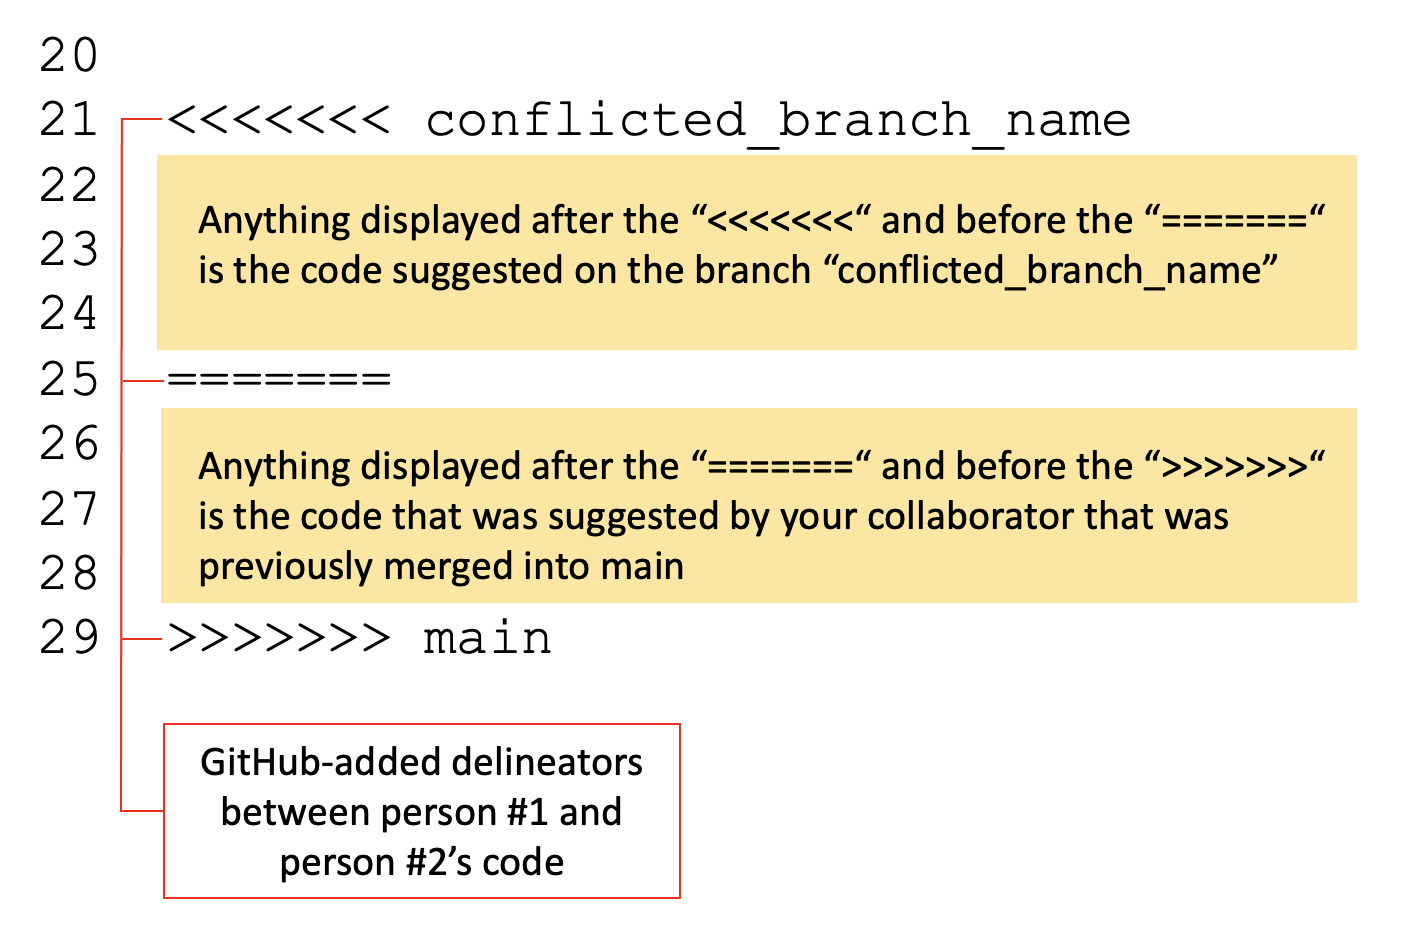
\includegraphics[width=0.75\linewidth]{./figures/Example-merge-conflict-github}

\hypertarget{practicing-a-merge-conflict-5}{%
\section{Practicing a merge conflict}\label{practicing-a-merge-conflict-5}}

\textbf{Both}: Together, look at the code in the file. Decide which edits you will keep. For this exercise, it is abritrary which edits you keep. However, keep in mind that in real life you will make this decision in an informed way.

When you choose what to keep, take out all of the \texttt{\textgreater{}\textgreater{}\textgreater{}} and \texttt{===} and \texttt{\textless{}\textless{}\textless{}} lines, as well as the lines from the person whose code you are not keeping. When you are finished, click \texttt{Mark\ as\ resolved} in the top right corner.

Note: You are still doing all of this on GitHub, not in your terminal.

\hypertarget{practicing-a-merge-conflict-6}{%
\section{Practicing a merge conflict}\label{practicing-a-merge-conflict-6}}

Now that you have clicked \texttt{Mark\ as\ resolved}, you will see a green checkmark next to the file name, and it will say \texttt{Resolved} in the top right corner. There will also be a green button in the top right corner that says \texttt{Commit\ merge}. Click on this button.

This brings you back to the page you are familiar with, where you can merge into main. Click \texttt{Merge\ pull\ request} and then \texttt{Confirm\ merge}. You can delete the branch as you usually do.

You have just resolved your first merge conflict!

\textbf{CR/LBW: add conclusion slides}
\textbf{make sure to mention that if all else fails, they should blow up their repo.}

  \bibliography{book.bib,packages.bib}

\end{document}
